\section{Visitor}

O padrão Visitor define uma estrutura que permite realizar 
operações em uma estrutura de objetos sem precisar alterá-los 
e sem precisar que os objetos dessa estrutura conheçam as 
operações que estão sendo realizadas. 

Uma estrutura alvo de um Visitor pode possuir objetos de 
classes diferentes. Por isso, o padrão deve implementar 
uma operação \textit{visit} para cada uma dessas classes, 
através de uma sobrecarga de métodos. Para que essa 
abordagem funcione, as classes da estrutura devem implementar 
uma operação \textit{accept} que recebe como parâmetro um 
Visitor genérico e chama sua operação \textit{visit}, 
passando uma referência para a instância atual (this) 
como parâmetro. Dessa forma, a função chamada é a 
que recebe a classe em questão como parâmetro.

Esse padrão permite estender objetos para novas operações 
sem comprometer sua implementação ou poluir as classes com 
diversas operações que não são de sua responsabilidade. 
Sua estrutura pode ser vista na imagem \ref{visitor_struct}.

\begin{figure}[htb]
	\caption{\label{visitor_struct}Estrutura do Visitor}
	\begin{center}
	    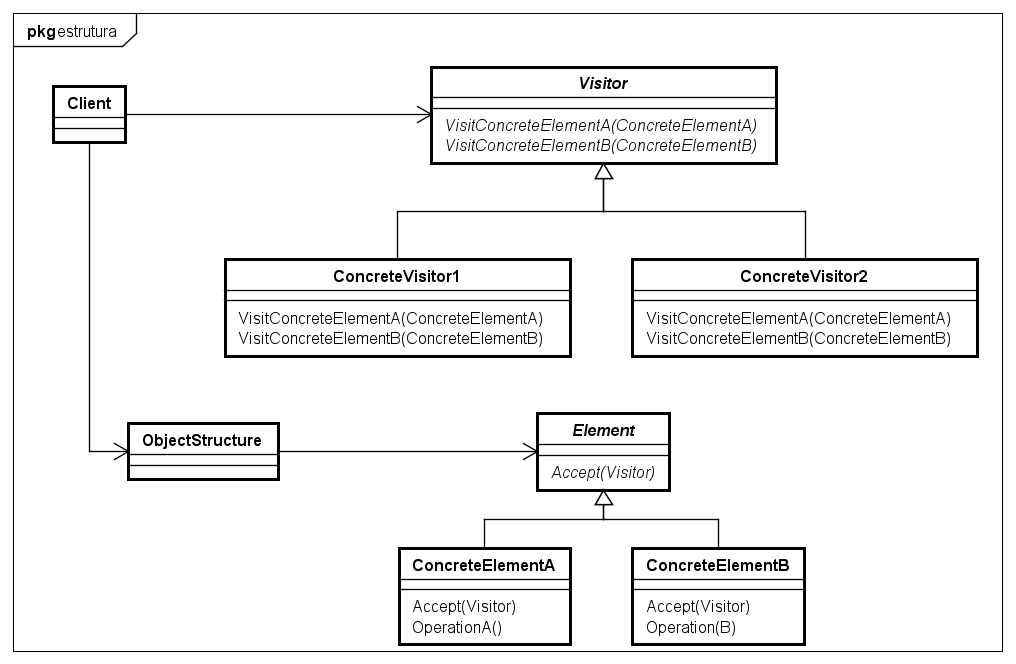
\includegraphics[scale=0.5]{5_padroes-contexto-funcional/5.3_comportamentais/5.3.11_visitor/visitor_estrutura.png}
	\end{center}
\end{figure}

\subsection*{Exemplo Orientado a Objetos}

Um compilador precisa fazer a análise de árvore abstrata sintática de 
um programa. Essa análise inclui diversas operações diferentes, como 
checagem de tipos e geração de código. Para que os nós da árvore 
não precisem implementar essas operações, elas implementam uma operação 
genérica que recebe como parâmetro qualquer Visitor. Dessa forma, para 
cada operação desejada, basta implementar uma nova classe Visitor 
que percorrerá os elementos da árvore abstrata sintática. O diagrama 
de classes para o exemplo pode ser visto na imagem \ref{visitor_exemplo1}, 
enquanto a implementação pode ser vista no código \ref{oovisitor}.

\begin{figure}[htb]
	\caption{\label{visitor_exemplo1}Exemplo de Visitor}
	\begin{center}
	    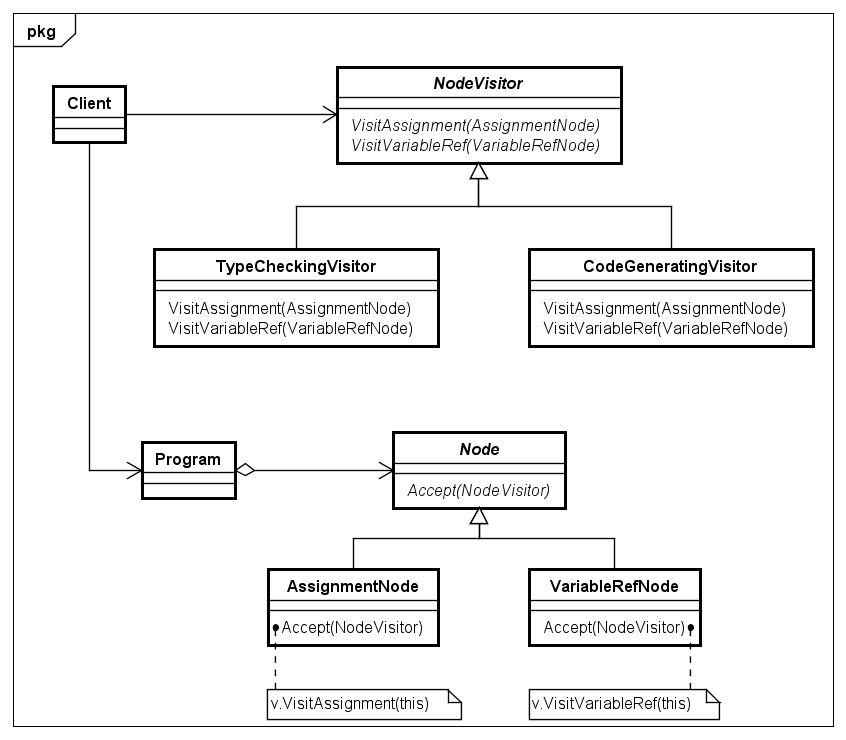
\includegraphics[scale=0.5]{5_padroes-contexto-funcional/5.3_comportamentais/5.3.11_visitor/visitor_exemplo.png}
	\end{center}
\end{figure}

\begin{lstlisting}[caption={Visitor Orientação a Objetos},label=oovisitor]

trait NodeVisitor {
  def VisitAssignment(node : AssignmentNode)
  def VisitVariableRef(node : VariableRefNode)
}

trait Node {
  def Accept(visitor : NodeVisitor)
}

class AssignmentNode extends Node {
  def Accept(visitor: NodeVisitor): Unit = visitor.VisitAssignment(this)
}

class VariableRefNode extends Node {
  def Accept(visitor : NodeVisitor) : Unit = visitor.VisitVariableRef(this)
}

class TypeCheckingVisitor extends NodeVisitor {

  def VisitAssignment(node: AssignmentNode): Unit = {
    //Operações de checagem de tipo para atribuição
  }

  def VisitVariableRef(node: VariableRefNode): Unit = {
    //Operações de checagem de tipo para variáveis
  }
}

class CodeGeneratingVisitor extends NodeVisitor {

  def VisitAssignment(node: AssignmentNode): Unit = {
    //Operações de geração de código para atribuição
  }

  def VisitVariableRef(node: VariableRefNode): Unit = {
    //Operações de geração de código para variáveis
  }
}

\end{lstlisting}

\subsection*{Contexto Funcional}

\begin{comment}
att
O Visitor é mais um caso em que funções de alta ordem ajudam a 
economizar novas classes e interfaces. Basta definir uma função 
que receba como parâmetro um valor do tipo encapsulado pela 
coleção e retornar um valor do mesmo tipo com a operação 
realizada. Funções do tipo map, que podem ser usadas para 
realizar uma operação em uma coleção, contribuem para essa 
implementação.

Porém, a funcionalidade do Visitor que permite realizar 
operações diferentes dependendo da implementação do objeto 
também é interessante e pode ser alcançada utilizando 
pattern matching. [terminar esse texto]
\end{comment}

\begin{lstlisting}[caption={Visitor Funcional},label=fpvisitor]
    

    
\end{lstlisting}